\documentclass[11pt,pdf,hyperref=unicode,hyperref={bookmarks=false}]{beamer}

\usepackage{cmap}
\usepackage[T2A]{fontenc}
\usepackage[utf8]{inputenc}
\usepackage[english,russian]{babel}

\usetheme{Goettingen}
%\usecolortheme{dove}

\author{Чистяков Александр}
\institute{группа 5126}
\title[Обзор научных статей]{Методология научных исследований\\ Обзор научных статей}

\begin{document}
    \begin{frame}
        \maketitle
    \end{frame}
    \begin{frame}{План}
        \tableofcontents
    \end{frame}
    \section{When Only Random Testing Will Do}
        \begin{frame}{When Only Random Testing Will Do}
            \begin{description}
                \item[Автор] Dick Hamlet
                \item[Издание] ACM New York, NY, USA 
                \item[Дата пуб.] 2006-07-17
                \item[Публикация] Proceedings of the First International Workshop on Random Testing (RT’06)
            \end{description}
Анализ областей, в которых Random testing оказывается эффективнее структурированного.
        \end{frame}
        \begin{frame}{Об авторе}
            \begin{center}
                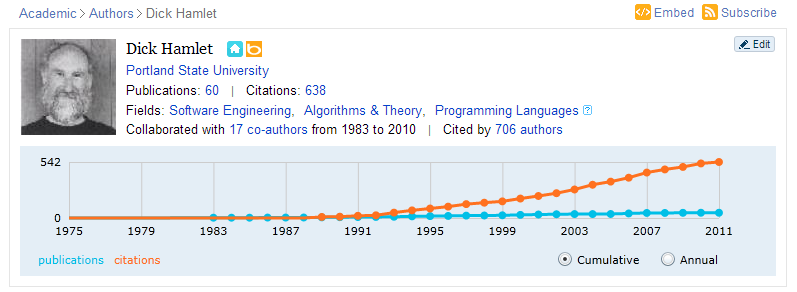
\includegraphics[keepaspectratio=true,width=\textwidth,height=0.8\textheight]{hamlet3.png}\\
            \end{center}
        \end{frame}
    \section{Finding Faults: Manual Testing vs. Random Testing+ vs. User Reports}
        \begin{frame}{Finding Faults: Manual Testing vs. Random Testing+ vs. User Reports}
            \begin{description}
                \item[Авторы] \begin{itemize} \item Ilinca Ciupa\item Bertrand Meyer\item Manuel Oriol\item Alexander Pretschner\end{itemize}
                \item[Издательство] Department of Computer Science,\\ETH Zurich, Switzerland
            \end{description}
Статистическое сравнение дефектов, найденных разными методами.
        \end{frame}
        \begin{frame}[allowframebreaks]{Об авторах}
            \begin{itemize}
                \item Ilinca Ciupa \\ 
                        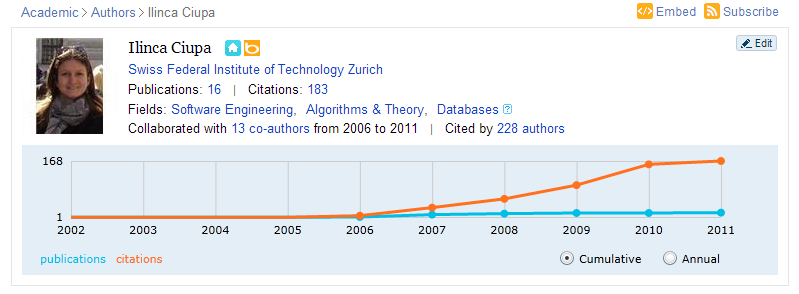
\includegraphics[keepaspectratio=true,width=0.9\textwidth,height=\textheight]{ciupa.png}\\
                        \framebreak
                \item Bertrand Meyer\\ 
                        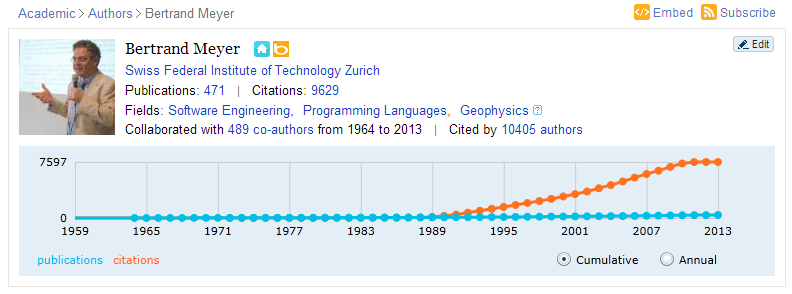
\includegraphics[keepaspectratio=true,width=0.9\textwidth,height=\textheight]{meyer.png}\\
                        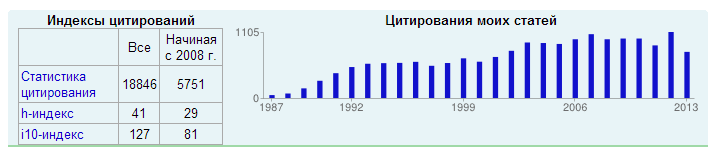
\includegraphics[keepaspectratio=true,width=0.9\textwidth,height=\textheight]{meyer2.png}\\
                        \framebreak
                \item Manuel Oriol\\ 
                        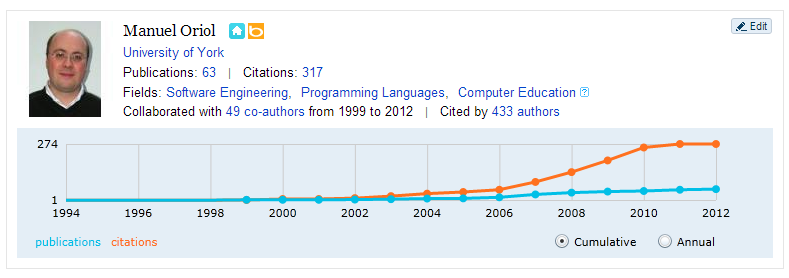
\includegraphics[keepaspectratio=true,width=0.9\textwidth,height=\textheight]{oriol.png}\\
                        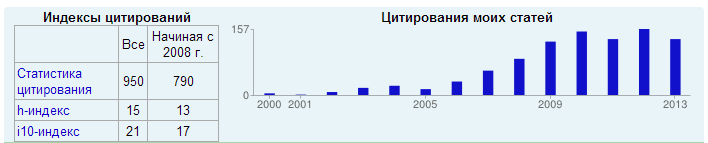
\includegraphics[keepaspectratio=true,width=0.9\textwidth,height=\textheight]{oriol2.png}\\
                        \framebreak
                \item Alexander Pretschner \\ 
                        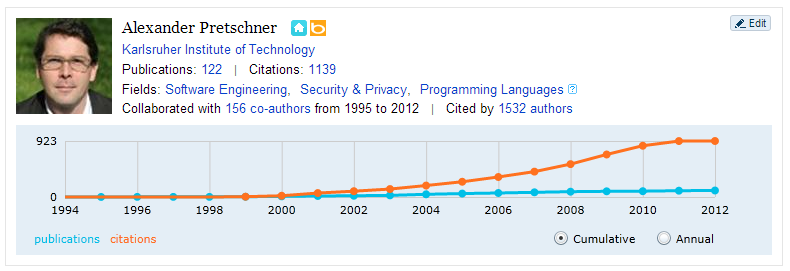
\includegraphics[keepaspectratio=true,width=0.9\textwidth,height=\textheight]{pretshner.PNG}\\
                        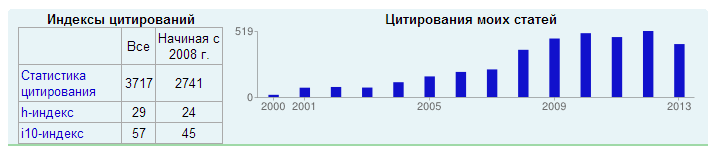
\includegraphics[keepaspectratio=true,width=0.9\textwidth,height=\textheight]{pretshner2.PNG}\\
            \end{itemize}
        \end{frame}
    \section{Experimental Assessment of Random Testing for Object-Oriented Software}
        \begin{frame}{Experimental Assessment of Random Testing for Object-Oriented Software}
            \begin{description}
                \item[Авторы] \begin{itemize} \item Ilinca Ciupa\item Andreas Leitner\item Manuel Oriol\item Bertrand Meyer\item Ilinca Ciupa \end{itemize}
                \item[Издание] ACM New York, NY, USA 
                \item[Дата пуб.] 2007-07-09
                \item[Публикация] ISSTA'07 Proceedings of the 2007 international symposium on Software testing and analysis
            \end{description}
Приминение Random testing к реальным проектам.
        \end{frame}
        \begin{frame}{Об авторах}
            \begin{itemize}
                \item Andreas Leitner\\ 
                        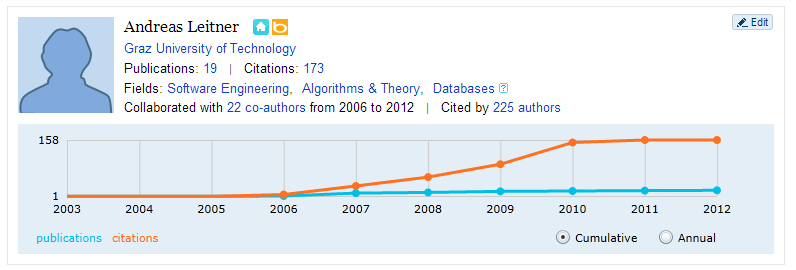
\includegraphics[keepaspectratio=true,width=0.9\textwidth,height=\textheight]{leitner.png}\\
            \end{itemize}
        \end{frame}
\section{}
\begin{frame}
    \begin{center}
        {\Large Спасибо за внимание!}
    \end{center}
\end{frame}
\end{document}
